%!TEX root = ../thesis.tex

\chapter{Motivation for top partner searches}
\label{ch:motivations}

Supersymmetry (SUSY)\cite{Borschensky:2014cia, Golfand:1971iw,, Volkov:1973ix, Wess:1974tw, Salam:1974ig} is a proposed extension of the SM.  It was first proposed as a feature of an early version of string theory, but then developed as a solution to the hierarchy problem.  In SUSY there is a boson partner to each fermion in the SM and vice-versa.  This means that there is a scalar partner to the top quark, called the stop quark ($\tilde{t}$)\footnote{Just as there are left- and right-handed quarks in the SM, there are left- and right-handed SUSY partners, $\tilde{t}_L$ and $\tilde{t}_R$ respectively.  These mix to form stop eigenstates, the lightest being $\tilde{t}_1$ and the heavier $\tilde{t}_2$.  The lighter $\tilde{t}_1$ is referred to as the $\tilde{t}$.} that cancels the large correction from the top quark.  The naming conventions for the SUSY particles are described in Section \ref{sec:PartCont}.  There are similar partners for the other quarks.  \\


%\subsection{Supermultiplets}

With this symmetry there is a transformation that turns a bosonic state to a fermionic one and vice versa; an operator, $Q$, that generates such a transformation with:

\begin{alignat}{2}
	Q|Fermion\rangle=&|Boson\rangle,\quad& Q|Boson\rangle=&|Fermion\rangle
\end{alignat}


The fermion and boson states that are transformed to one another by $Q$ come in pairs (called \textit{supermultiplets}) where the boson and fermion states are \textit{superpartners} of each other have the same mass, as well as the same electric charge, weak isospin, and color degrees of freedom.  Additionally, the number of fermionic and bosonic degrees of freedom in a supermultiplet must be equal. \\ %This means that for the simplest theory with one SUSY transformation, called the Minimal Supersymmetric Supersymmetry Model (MSSM), following combinations of supermultiplets are possible, from most to least simple \cite{susyprimer}: the \textit{chiral/matter/scalar} multiplet consisting of a Weyl fermion (two spin helicity states) and two real scalars (each with one degree of freedom); the \textit{gauge/vector} multiplet with two degrees of freedom consisting of a massless gauge boson (two helicity states) and a Weyl spin-1/2 fermion; and a gravatino supermultiplet, consisting of a spin-2 graviton (two helicity states) and a massless spin-3/2 gravatino (two helicity states). \\  %Any other combination will reduce to these for the so-called Minimal Supersymmetric Supersymmetry Model, or MSSM where there is only one Q.  Other ``extended" supersymmetric theories do not reduce to these supermultiplets.  \\


% Keep context in mind here
%Reference previous results, how ATLAS and CMS differ


%The Standard Model, as previously discussed, is an astoundingly accurate theory describing nature.  However the SM has several major shortfalls; among them are the hierarchy problem, what makes up dark matter, and failing to unify the gauge forces.  A theoretical solution to these three problems can be found in supersymmetry .   

The first three sections of this chapter will describe how SUSY is a solution to the major problems discussed in Chapter \ref{ch:intro}.  Then additional considerations of SUSY will be discussed, including more details about the particles it introduces and how it is broken, and then introduce a specific SUSY theory and how it is searched for at ATLAS.


\section{Hierarchy Problem}%Top Partners} 

As discussed in Section \ref{sec:HierarchyProblem}, one-loop corrections to the Higgs mass results in large divergences.  One solution is to introduce additional physics that adds diagrams to cancel the troublesome diagrams, as:

\begin{equation}
\begin{tikzpicture}
\begin{feynman}[inline=(a.base)]
\diagram [horizontal=a to b, layered layout] {
	a -- [scalar] b -- [scalar] c
};
\draw [scalar] (b) arc [start angle=270, end angle=-90, radius=0.5cm] node[midway, above] {$\tilde{t}$}; % {\stop};
\end{feynman}
\end{tikzpicture}
= +\frac{\lambda_f^2}{8\pi^2}\Lambda_{\mathrm{UV}}^2
\label{eq:stoploop}
\end{equation} 

This is because the sign difference between the fermion and scalar loops leads to the cancellation of the fermion loops and also persists to higher order loop corrections.  The existence of such scalars arises naturally if there exists a symmetry relating bosons to fermions, as in SUSY.  



%%%%%%%%%%%%%%%%%%%%%%%%%%%%%%

%\section{Supersymmetry}


% R parity
\section{Dark Matter}

In some SUSY models lepton and baryon numbers can be violated, which results in the lifetime of a proton being shorter than observed\cite{SuperK}.  It is not desirable to simply take baryon and lepton conservation as a postulate because it is a consequence of the SM.  However a new symmetry, called ``matter parity" can be introduced, defined as:

\begin{equation}
P_{M} = (-1)^{3(B-L)}
\end{equation}

where B and L are the baryon and lepton numbers respectively, for each particle in the theory.  Quark and lepton supermultiplets have $P_M=-1$ while the Higgs supermultiplets have $P_M=+1$.  Gauge bosons and gauginos, which do not have baryon or lepton number, are assigned $P_M=+1$.  A candidate term in the Lagrangian is only allowed if the product of all $P_M$ terms is +1.  This is a more exact and fundamental theory than baryon and lepton number conservation.  A new symmetry, ``$R$-parity,"\cite{FARRAR1978575} can be introduced to also account for conservation of spin as:

\begin{equation}
P_{R} = (-1)^{3(B-L) + 2s}
\end{equation}

where $s$ is the spin of the particle.  All the particles in the SM have positive, or even, $R$-parity, while all SUSY particles have negative, or odd, $R$-parity.  If $R$-parity is exactly conserved then there is no mixing between SM and SUSY particles.  Additionally, the lightest supersymmetric particle must be stable since it cannot decay to SM particles. \\

The upshot of $R$-party is that SUSY naturally provides a viable dark matter candidate\cite{ELLIS1984453}, giving a solution to the second major problem in the SM.  In the early universe when the temperature cooled, dark matter particles no longer had the energy to annihilate with each other to produce SM particles and also could not decay directly into SM particles, leaving a relic density of dark matter particles.



% gauge coupling unification (add figure 6.8 in primer)

\section{Gauge Coupling Unification}

The third major problem in the SM, that the SM the gauge couplings unify at some energy scale, also has a solution in SUSY.  In some SUSY models the three gauge coupling constants are unified at an energy scale of $10^{15}$ or $10^{16}$ GeV.  This is referred to as the grand unified theory (GUT) scale.  The unification is not exact but very close, as seen in Figure \ref{fig:unification} and adjustments can be made approaching the GUT scale.  

\begin{figure}[tbh]
	\centering
	\includegraphics[width=.7\textwidth,trim={0 0 0 0},clip]{gaugeunification}
	\caption[Gauge coupling unification]{Renormalization group evolution of inverse gauge couplings in the Standard Model (dashed) and with a SUSY theory (solid) with varying SUSY particle mass thresholds and couplings.  The SM couplings do not unify at any point while the MSSM couplings nearly unify at an energy scale of $10^{16}$ GeV (figure from \cite{susyprimer}).} }
	\label{fig:unification}
\end{figure}


%\subsection{Simplified Models} %https://arxiv.org/pdf/0810.3921.pdf
%
%It's not feasible to scan the complete space SUSY models because of the large parameter space available.  Also searching for a more specific model such as GMSB is also not feasible since it does not allow for mass reordering.  Therefore simplified models are used with only a few parameters to vary and several benchmark mass points.  This gives a good coarse-level description of SUSY physics and deviations from the models can be used to characterize underlying physics.  Generally a simplified model will have just one pair-produced species of particles and only a few steps in the decay chain.  Doing this makes developing search strategies and interpreting results easier.  \\
%
%Results from simplified models can then be reinterpreted for more complex models.  For example, Phenomenological MSSM (pMSSM) uses theoretical assumptions and experimental results to motivate reducing the number of free parameters from 105 to 19.  Each set of values for the 19 values is a model point and models can be excluded by sampling the parameter grid and applying results of analysis.  \\

%MOVE below introduction to susy

% searching for susy/mass spectrum:




\section{Particle Contents}
\label{sec:PartCont}

Only chiral supermultiplets can contain fermions whose left- and right-handed parts transform differently under the gauge group; since all the SM fermions have this property they must be members of the chiral multiplet and therefore the bosonic partners must be scalar particles, called \textit{sfermions}, named by adding an s (for ``scalar") in front of the standard model particle name, and not spin-1 vector particles.  All supersymmetric particles are noted by a tilde ($\sim$) over its letter symbolizing it.  The squarks in the first and second families are nearly degenerate (due to smaller Yukawa couplings compared to the third generation) and are much heavier than the sleptons.  The stop quark is expected to be the lightest squark as the large Yukawa couplings tend to drive down the masses of the third generation squarks in the renormalization group equations faster than the first two generations\cite{susyprimer}.  As the masses of the third generation families increase, SUSY becomes less natural and the motivation for SUSY as a solution to the hierarchy problem diminishes.  \\%due to large radiative corrections from loops with the gluino, and cannot be much lighter than the mass of the gluino.  \\

Alternately, there must be at least two chiral supermultiplet for the Higgs, one to couple to up-type quarks ($H_u^+ , H_u^0$) and one to couple to down-type quarks and charged leptons ($H_d^0, H_d^-$).  Each of these have a spin-1/2 partner, named by adding ``-ino" to the end of the standard model partner, so are named \textit{higgsinos}.  \\

Finally, the gauge bosons  have gauge supermultiplets with spin-1/2 superpartners.  Similarly to the Higgs, the naming convention is to add ``-ino" to the end of the standard model partner, so are named \textit{gauginos}.  The partner for the gluon is the \textit{gluino} and the partners for the \textit{W} and \textit{B} bosons are the \textit{winos} and \textit{bino}.  Because of electroweak symmetry breaking, the winos and binos mix to make the zino and photino.  The higgsinos and electroweak gauginos mix with each other  similarly to the $W$ and $B$ bosons mixing in the SM.  Also the neutral higgsinos ($\widetilde{H}^0_u,\widetilde{H}^0_d$)  mix with the neutral gauginos ($\widetilde{W}^0$, $\widetilde{B}$) to create four neutral mass eigenstates called neutralinos, $\widetilde{\chi}^0_1-\widetilde{\chi}^0_4$, while the charged higgsinos and winos mix to form four charginos, $\widetilde{\chi}^\pm_1-\widetilde{\chi}^\pm_4$.  The lightest neutralino, $\widetilde{\chi}^0_1$, is the lightest supersymmetric particle (LSP) and is a candidate for dark matter.  \\

The decay of a squark to a quark and gluino will dominate if kinematically allowed.  Otherwise squarks can decay to a quark and neutralino or chargino, and the decay to a quark and LSP is kinematically favored and can dominate for right-handed squarks if the LSP is mostly bino.  Left-handed squarks may prefer decaying to heavier neutralinos and charginos depending on the coupling to winos compared to binos.  \\

Table \ref{tab:smsusypartners} shows the superpartners of the SM particles.  \\



\begin{table}[!htb]
	\centering
	\begin{tabular}{c|c}
		\hline
		%\multicolumn{2}{c|}{Field components}				\\%			& \multirow{2}{*}{Comments} \\
		\cline{2-3}
									 \Gls{SM} 										& \Gls{SUSY} partners															 \\
		\hline\hline
		\multicolumn{5}{c}{Spin-1/2 quarks and spin-0 squarks} \\
		\hline
		$\begin{pmatrix} u_L&d_L\end{pmatrix}$		& $\begin{pmatrix} \tilde{u}_L&\tilde{d}_L\end{pmatrix}$					\\ %& \multirow{3}{*}{$\times3$ generations}\\
		 $u^{\dagger}_R$								& $\tilde{u}^*_R$														& \\
		 $d^{\dagger}_R$								& $\tilde{d}^*_R$														& \\
		\hline\hline
		\multicolumn{5}{c}{Spin-1/2 leptons and spin-0 sleptons} \\
		\hline
		$\begin{pmatrix} \nu_L&e_L\end{pmatrix}$		& $\begin{pmatrix} \tilde{\nu}_L&\tilde{e}_L\end{pmatrix}$				\\	%& \multirow{2}{*}{$\times3$ generations}\\
		$e^{\dagger}_R$								& $\tilde{e}^*_R$														\\%& \\
		\hline\hline
		\multicolumn{5}{c}{Spin-0 Higgs and spin-1/2 Higgsinos} \\
		\hline
		$\begin{pmatrix} H_u^+&H_u^0\end{pmatrix}$	& $\begin{pmatrix} \widetilde{H}_u^+&\widetilde{H}_u^0\end{pmatrix}$		\\%& \\
		$\begin{pmatrix} H_d^0&H_d^-\end{pmatrix}$	& $\begin{pmatrix} \widetilde{H}_d^0&\widetilde{H}_d^-\end{pmatrix}$		\\%& \\
		\hline\hline
		\multicolumn{5}{c}{Spin-1 gauge bosons and spin-1/2 gauginos} \\
		\hline
		$g$											& $\tilde{g}$											\\%& \\
		$\begin{pmatrix} W^{\pm}&W^0\end{pmatrix}$	& $\begin{pmatrix} \widetilde{W}^{\pm}&\widetilde{W}^0\end{pmatrix}$						\\%& \\
		$B^0$											& $\widetilde{B}^0$												\\%& \\
		\hline\hline
	\end{tabular}
	\caption{Standard Model particles and their associated superpartners.}
	\label{tab:smsusypartners}
\end{table}


\section{Supersymmetry Breaking}

Particles in mutiplets will have the same mass in an unbroken supersymmetry; because this is not the case, as sparticles would have been easily discovered, supersymmetry is a broken symmetry in the vacuum state.  Specifically, it must be broken \textit{spontaneously}, meaning that the underlying model is invariant under supersymmetry but the vacuum state is not.  This way supersymmetry is hidden at low energies.  Since the relationship between the dimensionless couplings of the SM and supersymmetry has to be maintained in order for supersymmetry to be a solution to the hierarchy problem, the idea of ``soft" supersymmetry breaking in introduced.  The soft terms introduce new Higgs mass corrections as\cite{susyprimer}:

%where $\Lagr_{\mathrm{SUSY}}$ contains all couplings and Yukawa interactions and preserves supersymmetry invariance and $\Lagr_{\mathrm{soft}}$ contains only mass terms and coupling parameters with positive mass dimension to naturally maintain a hierarchy between the electroweak scale and Planck scale.  


\begin{equation}
	\Delta m_H^2 = m_{\mathrm{soft}}^2 \left[ \frac{\lambda}{16\pi^2}\ln(\Lambda_{\mathrm{UV}}/m_{\mathrm{soft}})+\dots \right]
\end{equation}

where $\lambda$ is a dimensionless coupling term and $m_{\mathrm{soft}}$ is the mass scale associated with the soft terms.  Since the masses of the fermion and their superpartners are not equal the additional diagrams do not perfectly cancel the divergent diagrams.  In order to be a viable solution to the hierarchy problem the soft mass term, and thus the lightest supersymmetric particles, should be on the order of the TeV scale.\\% and not too much larger in order to maintain $\sim$1\% fine-tuning.  \\

%breaking scale

There are two primary competing proposals for what the mediating interactions may be.  The first is new physics that enter at the Planck scale, including gravity, called the Planck-scale-mediated supersymmetry breaking (PMSB).  The second proposal is that the interactions for SUSY breaking are the electroweak and QCD gauge interactions in the SM, called gauge-mediated supersymmetry breaking (GMSB).\footnote{There is also a possibility that the sectors are geographical; in this proposal there are extra spatial dimensions that are of the Kaluza-Klein type or warped type so that there is a physical distance that separates the visible and hidden sectors.  This can fit with string theory which suggests six extra spatial dimensions.} \\ %In this scenario SUSY is broken in the hidden sector by a VEV ($\langle F \rangle$) and the soft terms are roughly $m_{soft} \sim \langle F \rangle/M_{P}$ because $m_{soft}$ must disappear as $\langle F \rangle \rightarrow 0$ where SUSY is unbroken and the limit where $M_{P} \rightarrow \infty$ where gravity is irrelevant.  If $m_{soft}$ is a few hundred GeV then $\langle F \rangle \sim 10^{10}$ or $10^{11}$ GeV. \\

%The second proposal is that the flavor-bind mediating interactions for SUSY breaking are the electroweak and QCD gauge interactions in the SM, called gauge-mediated supersymmetry breaking (GMSB).  In this scenario the MSSM soft terms come from loop diagrams involving some messenger particles that are new chiral supermultiplets that couple to the SUSY-breaking VEV ($\langle F \rangle$).   Then for the MSSM soft terms,  $m_{soft} \sim \frac{\alpha_{a}}{4\pi}\frac{\langle F \rangle}{M_{\mathrm{mess}}}$ where $M_{\mathrm{mess}}$ is the mass of the messenger particles, and if $M_{\mathrm{mess}}$ and $\sqrt{\langle F \rangle}$ are comparable then the SUSY scale can be as low as $\langle F \rangle \sim 10^4$ GeV, which is clearly lower than the gravity-mediated case and gives $m_{\mathrm{soft}}$ the right order of magnitude. \\

%% soft lagran

% Mass spectrum

\section{Minimal Supersymmetric Standard Model} %and Phenomenological MSSM }


As previously discussed, the number of fermionic and bosonic degrees of freedom in a supermultiplet must be equal.  This means that for the simplest theory with one SUSY transformation ($Q$), called the Minimal Supersymmetric Standard Model (MSSM)\cite{Djouadi:1998di}, the following combinations of supermultiplets are possible, from most to least simple: the \textit{chiral/matter/scalar} multiplet consisting of a Weyl fermion (two spin helicity states) and two real scalars (each with one degree of freedom); the \textit{gauge/vector} multiplet with two degrees of freedom consisting of a massless gauge boson (two helicity states) and a Weyl spin-1/2 fermion; and a gravatino supermultiplet, consisting of a spin-2 graviton (two helicity states) and a massless spin-3/2 gravatino (two helicity states).  Any other combination will reduce to these for the MSSM.  Other ``extended" supersymmetric theories do not reduce to these supermultiplets.  \\

After SUSY breaking, the MSSM adds 105 masses, phases and mixing angles that do not have a counterpart in the ordinary SM, so SUSY breaking introduces an arbitrariness to the theory.  One way to handle this is called phenomenological MSSM, or pMSSM.


\section{Phenomenological MSSM}
\label{sec:pmssm}

These parameters are reduced in the pMSSM\cite{pMSSM} by applying experimental and theoretical constraints to narrow the number to 19.  These constraints include assuming $R$-parity is conserved, that the LSP is the lightest neutralino, that there is no new CP-violation in the SUSY sector, and no extra flavor changing neutral currents.  In addition to these experimental results from electroweak and flavor measurements and searched at LEP and the Tevatron are imposed.  Figure \ref{fig:pmssm} illustrates how the MSSM and pMSSM fit together in the larger SUSY theory. \\

\begin{figure}
\centering
	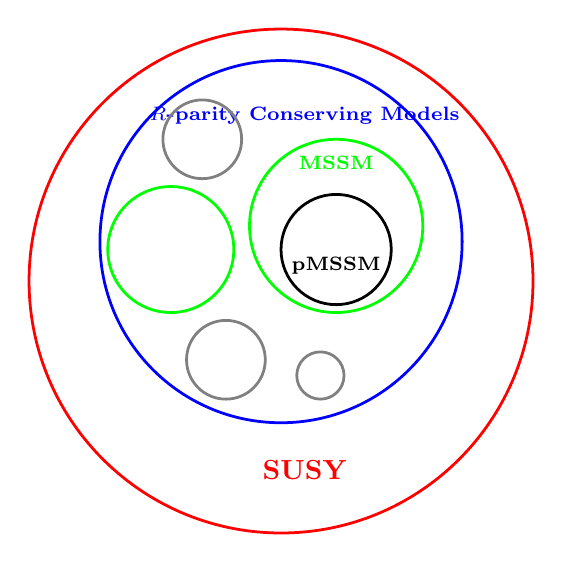
\begin{tikzpicture}
        \draw[draw=red, line width=1] (4.9,2.4) arc(0:360:3.2 and 3.2);
        \node[align=center,red,font={\bfseries}] at (2,0) {SUSY};
        
        \draw[draw=blue, line width=1] (4,2.9) arc(0:360:2.3 and 2.3);
        \node[align=center,blue,font={\scriptsize\bfseries}] at (2.,4.5) {$R$-parity Conserving Models};%N=1};

        \draw[draw=green, line width=1] (3.5,3.1) arc(0:360:1.1 and 1.1);
        \node[align=center,green,font={\scriptsize\bfseries}] at (2.4,3.9) {MSSM};
        \draw[draw=green, line width=1] (1.1,2.8) arc(0:360:0.8 and 0.8);
        \node[align=center,green,font={\scriptsize\bfseries}] at (0.4,2.6) {};%NMSSM};

        \draw[draw=black, line width=1] (3.1,2.8) arc(0:360:0.7 and 0.7);
        \node[align=center,black,font={\scriptsize\bfseries}] at (2.4,2.6) {pMSSM};
        \draw[draw=gray, line width=1] (1.5,1.4) arc(0:360:0.5 and 0.5);
        \draw[draw=gray, line width=1] (2.5,1.2) arc(0:360:0.3 and 0.3);
        \draw[draw=gray, line width=1] (1.2,4.2) arc(0:360:0.5 and 0.5);

        %\node[black,font={\tiny}] at (2,-1.3) {T. Rizzo, SLAC Summer Institute 2012};
          \end{tikzpicture} 
          
\caption[Illustration of the pMSSM as a subset of SUSY theories]{An illustration of the pMSSM as a subset of the larger MSSM, both under the larger umbrella of SUSY theories (figure based off of \cite{rizzossi2012}).}% with one SUSY transformation, N=1.} 
\label{fig:pmssm}
\end{figure}
%
%%\subsection{Mass Spectrum}
%%
%%In the MSSM there are two complex Higgs doublets rather than just one as in the SM.  Each get their own VEV as $\langle H_{u} \rangle = v_{u}$ and $\langle H_{d} \rangle = v_{d}$.  This are related to the mass of the {\Zboson} boson and electroweak gauge couplings as:
%%
%%\begin{equation}
%%v_u^2 + v_d^2 = v^2 = \frac{2m_{\Zboson}^2}{(g^2+g^{'2})} \approx (246 \mathrm{GeV})^2
%%\end{equation}
%%
%%with the ratio between the two \gls{vev}:
%%
%%\begin{equation}
%%\tan \beta \equiv \frac{v_u}{v_d}
%%\end{equation}
%%%\frac{\pi}{2}$.
%%
%%where both $v_u$ and $v_d$ are real and positive, and the value of $\tan \beta$ is not fixed by experiments but depends on Lagrangian parameters but must be $0 < \tan \beta < \frac{\pi}{2}$.  \\
%%
%%The Higgs scalar fields in the MSSM consist of eight real scalar degrees of freedom.  After electroweak symmetry breaking three of these are the Nambu-Goldstone bosons, $G^{0}$ and $G^{\pm}$, that become longitudinal modes of the $Z^0$ and $W^{\pm}$ bosons.  The other five degrees Higgs scalar mass eigenstates include two CP-even neutral scalars, $h^0$ and $H^0$, one CP-odd neutral scalar $A^0$, one charge +1 $H^+$, and one which is its conjugate $H^-$. The discovered $\sim 125$ GeV Higgs is usually assumed to be the lighter $h^0$. \\
%
%%%Electrowinos  
%%
%%  The exact mixing varies from model to model, so the mass and charge are the focus of experimental searches.  The lightest neutralino is assumed to be the lightest supersymmetric partner (LSP), unless there is a lighter gravitino or unless $R$-parity is not conserved, and is therefore the only particle in the MSSM that makes a good dark matter candidate.  \\
%%
%%% gluino
%%
%%The gluino is a color octet fermion and so cannot mix with any other particle in the MSSM. Its mass parameter, $M_{3}$ is related to the bino and wino mass parameters, $M_{1}$ and $M_{2}$ as $M_{3}:M_{2}:M_{1} \approx 6:2:1$ (following MSUGRA or GMSB boundary conditions) so the gluino is expected to be much heavier than the neutralinos and charginos.  \\
%%
%%% sfermions
%%
%%The squarks in the first and second families are nearly degenerate and are much heavier than the sleptons due to large radiative corrections from loops with the gluino, and cannot be much lighter than the mass of the gluino.  Additionally, left-handed sfermions are heavier than right-handed sfermions due to effects from the renormalization group.  The third family sfermions are most likely the lightest sfermions due to contributions from their renormalization group equations. \\
%
%%Potentially dangerous flavor-changing and CP-violating effects in the MSSM can be avoided if SUSY breaking is universal.  In the case where the squark and slepton squared-mass mixing angles are flavor-blind, and each proportional to the 3x3 identity matrix in family space, the squark and slepton mixing angles are trivial and SUSY contributions to flavor changing currents are very small.  Additionally, assuming the scalar couplings are proportional to the corresponding Yukawa coupling matrix ensures that only squarks and sleptons of the third family can have large scalar couplings.  Furthermore, large CP-violating effects can be avoided by assuming soft parameters do not introduce new complex phases.  These conditions make up a weak version of the soft supersymmetry-breaking universality hypothesis and has fewer parameters than the general case.  There are several alternatives to the universality hypothesis but add complexity or require very heavy masses. \\
%
%%\begin{figure}[tbh]
%%	\centering
%%	\includegraphics[width=.5\textwidth,trim={0 0 0 0},clip]{massspectrum}
%%	\caption{A possible mass spectrum for the MSSM.  This is one particular model for GMSB; different models vary greatly, including in mass scales, which is not shown.  \cite{susyprimer} \color{red}{Replace with higher resolution image.  Add other possible spectra?} }
%%	\label{fig:massspect}
%%\end{figure}
%% squark decays
%
%%The decay of a squark to a quark and gluino will dominate if kinematically allowed because it has QCD strength.  Otherwise squarks can decay to a quark and neutralino or chargino, and the decay to a quark and LSP is kinematically favored and can dominate for right-handed squarks if the LSP is mostly bino.  Left-handed squarks may prefer decaying to heavier neutralinos and charginos because the coupling to winos is stronger than binos.  \\
%
%
%\section{Simplified Models}
%
%While a new model of physics can involve many new and complex particles and interactions, simplified models are designed to only involve a few new particles and interactions.  These can be limits of more complex scenarios but with new particles integrated out and can be described by a few parameters related to collider physics, such as particle mass, production cross-sections, and branching fraction.  Figure \ref{fig:stopSimple} shows the simplified model in this search with a gray blob after the proton collision but before the stop production that represents model-specific physics that is integrated out for the simplified model.  This helps to avoid some of the limitations of model-dependent searches and sensitivity to new physics can be presented of a function of these few parameters and over full ranges of new particle masses.  The primary application for simplified model results are to identify the boundaries of search sensitivity, describing new physics signals, and deriving limits on more general models. \\
%
%In this search with $R$-parity conserving models the stop cross section is mostly decoupled from the model parameters\cite{Beenakker:1997ut, Beenakker:2010nq, Beenakker:2011fu, Borschensky:2014cia}.  The stop decay depends on the left- and right-handed stop mixing, the mass of the stop, and the mixing parameters of the charginos and neutralinos.  
%
%\begin{figure}[tbh]
%	\centering
%	\includegraphics[width=.4\textwidth,trim={0 0 0 0},clip]{stst-ttN1N1.pdf}
%	\caption{\label{fig:stopSimple}{Simplified models of stop pair production.  The gray blob after the proton collision represents a black box with potentially complex physics, which is integrated out.}}
%\end{figure}
%
%
%
%\subsection{Search for Direct Pair-Produced Stops}
%
%Because the stop quark is the lightest sfermion while also having the largest impact on fixing the hierarchy problem, searching for the stop is well-motivated.  Introducing $R$-parity preserves baryon and lepton number conservation while also providing a candidate for dark matter, which means that stop quarks are produced in pairs.  
%
%
%
%
%
%%As a scalar particle, the Higgs mass correction goes as:
% %Because the top quark is so much more massive than other fundamental particles (nearly 40 times heavier than the next heaviest fermion) and because of the large top Yukawa coupling,  its mass essentially sets the mass correction for the higgs. 
%
%%\begin{equation}
%%\feynmandiagram [inline=(a.base), layered layout, horizontal=b to c]
%%{ 
%%	a -- [scalar] b 
%%	-- [fermion, half left, looseness=1.6, edge label=\(t\)] c 
%%	-- [fermion, half left, looseness=1.6] b,
%%	c -- [scalar] d,
%%};
%%= -\frac{6y_t^2}{16\pi^2}\Lambda_{\mathrm{UV}}^2
%%\label{eq:toploop}
%%\end{equation}
%
